%version 1.00,	date 12/05/2016	auteur(s) Pierre Porche
\speaker{\Julie}

\begin{frame}
\frametitle{F5 : Aide à l'attribution des interventions}
	\begin{minipage}[c]{.40\linewidth}
      \begin{figure}[r]
		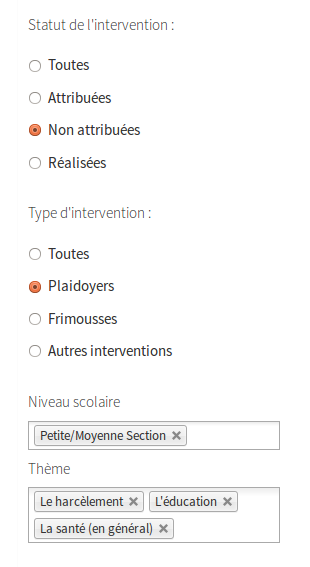
\includegraphics[scale=0.3]{images/filtreListeIntervention.png}
		\caption{Capture d'écran des possibilités de tris}
	  \end{figure}
   \end{minipage} \hfill
   \begin{minipage}[c]{.52\linewidth}
      \begin{block}{Les filtres}
		\begin{itemize}
			\item Requêtes sur la base de données
			\item Notion de \texttt{Repository}
		\end{itemize}
	  \end{block}
	  \begin{block}{Rôle des \texttt{Repository}}
		Un \texttt{Repository} permet de centraliser tout ce qui touche à la récupération des entités.
		\begin{itemize}
		\item \texttt{PHP class} 
		\item \texttt{extends EntityRepository}
		\end{itemize}
	  \end{block}
   \end{minipage} \hfill
\end{frame}

\begin{frame}
\frametitle{F5 : Aide à l'attribution des interventions}
	\begin{block}{Les méthodes de récupération des entités}
		\begin{itemize}
			\item Méthodes de récupération de base : \\
			 \texttt{find, findAll, findBy, findOneBy, findByX, findOneByX}
			\item Méthodes de récupération personnalisées : \\
			\begin{itemize}
			\item \texttt{DQL (Doctrine Query Language)} : SQL adapté à la vision objets
			\item \texttt{Query Builder}: construction de la requête étape par étape
			\end{itemize}			
		\end{itemize}
	  \end{block}
\end{frame}

\begin{frame}
\frametitle{F5 : Aide à l'attribution des interventions}
	\textbf{But :} récupérer les interventions attribuées au bénévole courant. \\
	\vskip 0.5cm
	\begin{block}{Requête SQL }	
	\texttt{ 
	%\noindent \textbackslash \texttt{set idUtilisateurCourant }\\
	SELECT \textcolor{red}{i}.* FROM intervention \textcolor{red}{i} \\
	\setlength{\parindent}{1cm}	WHERE \textcolor{red}{i}.id\_benevole = \textcolor{blue}{10};}
	\end{block}
	\begin{block}{Requête Query Builder }
	\noindent \texttt{\$qb = \$this->createQueryBuilder('\textcolor{red}{i}'); \\
	\noindent \$qb \\
	\setlength{\parindent}{1cm} ->where('\textcolor{red}{i}.benevole = :user') \\
    \setlength{\parindent}{1cm} ->setParameter('user', \textcolor{blue}{\$user});}
	\end{block}
\end{frame}

\begin{frame}
\frametitle{F6 : Attribution/réalisation d'une intervention}
      \begin{figure}[r]
		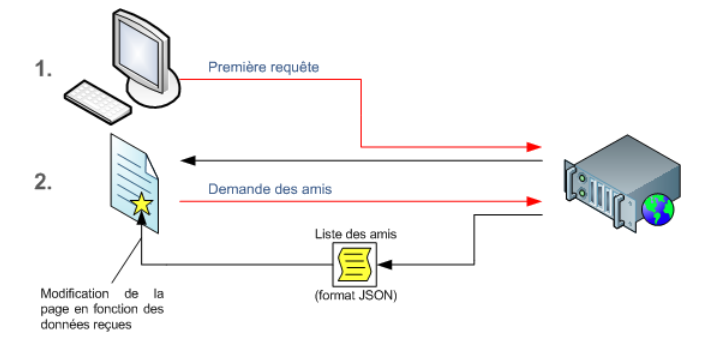
\includegraphics[scale=0.35]{images/ajax.png}
		\caption{Schéma explicatif d'AJAX}
	  \end{figure}
\end{frame}
